\subsection{Glyph: \glyph{Or}}
\label{sec:af:or}

The glyph \glyph{or} is used to denote that any of the \glyph{AFNs} linked as input is sufficient to produce the output.

\begin{glyphDescription}
 \glyphSboTerm SBO:0000174 ! or.
 \glyphOrigin More than one AFN (section~\ref{sec:af:ANs}) or logical operator (section~\ref{sec:af:logic}).
 \glyphTarget  A modulation arc (section~\ref{sec:af:arcs}). 
 \glyphNode \glyph{Or} is represented by a circle carrying the word ``OR''.
 \end{glyphDescription}

\begin{figure}[H]
  \centering
  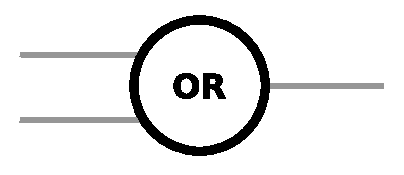
\includegraphics[scale = 0.5]{images/or}
  \caption{The \AF glyph for \glyph{or}. Only two inputs are represented, but more would be allowed.}
  \label{fig:af:or}
\end{figure}
